\begin{mybilan}
	\begin{itemize}
		
		\item Un objet ou un phénomène qui peut produire de l'énergie est une \kw{source d'énergie}.
				
		\item Il existe différentes \kw{formes d'énergie} :
		
			\begin{itemize}
				\item énergie cinétique (associée à un mouvement) ;
				\item énergie thermique ;
				\item énergie chimique ;
				\item énergie électrique ;
				\item énergie lumineuse.
			\end{itemize}
		
		\item Il existe deux catégories de formes d'énergie :
			\begin{itemize}
				\item Les sources d'énergie \kw{renouvelables} peuvent être utilisées de façon illimitée à l'échelle humaine.
				\item Les sources d'énergie \kw{non renouvelables} (ou fossiles) ont des stocks limités et ne peuvent pas se renouveler à l'échelle humaine.
			\end{itemize}
	\end{itemize}


	\begin{center}
		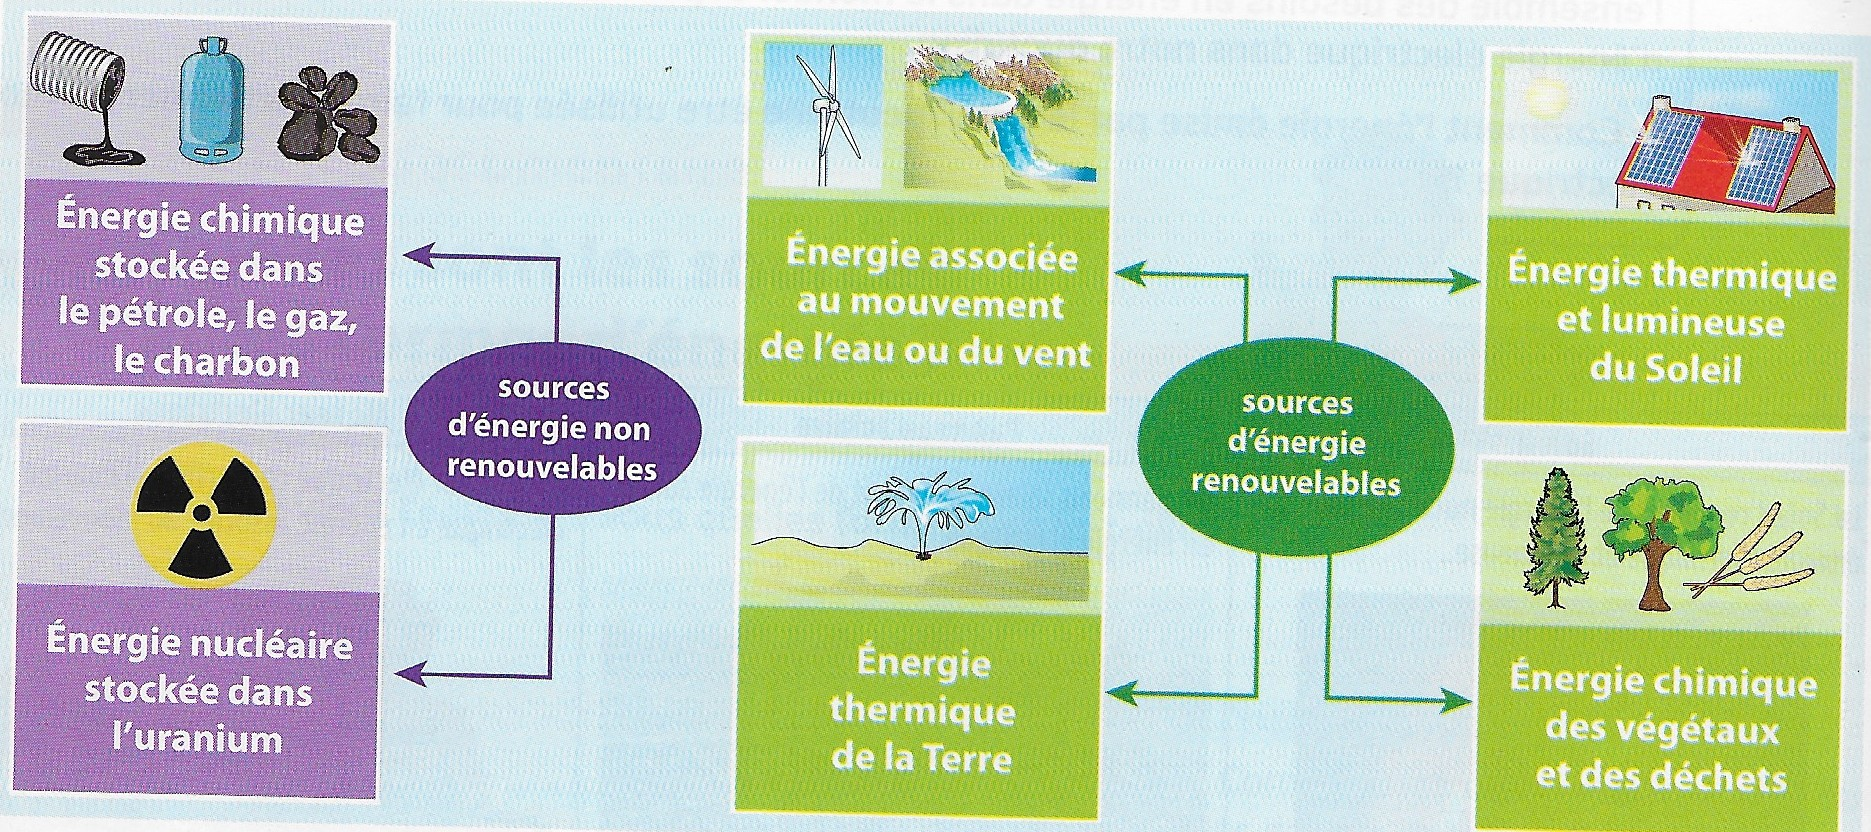
\includegraphics[scale=0.8]{img/types_energie}
	\end{center}
\end{mybilan}